\documentclass[14pt,a4paper]{extarticle}
%\documentclass[12pt,a4paper]{article}

\usepackage[utf8]{inputenc}
%\usepackage[ukrainian]{babel}


\usepackage{amssymb}
\usepackage{physics}


\usepackage[active]{srcltx}
\usepackage[final]{pdfpages}

\usepackage[hidelinks]{hyperref}

\usepackage{verbatim}

\usepackage[utf8]{inputenc}
\usepackage[active]{srcltx}
\usepackage[final]{pdfpages}
\usepackage[hidelinks]{hyperref}

\usepackage{verbatim}
\usepackage{amssymb}
\usepackage{physics}
\usepackage{amsmath}
\usepackage{algpseudocode}
\usepackage{algorithm}

\floatname{algorithm}{Algorithm}
%%%%%%%%%%%%%%%%%%%%%%%%%%%%%%%%%%%%%%%%%%%%%%%%%%%%%%%%%%%%%%%%%%
%\pagestyle{empty}                     %нумерацiя сторiнок i т.д.
\pagestyle{headings}                   %нумерацiя сторiнок вгорi зправа i т.д.
%\renewcommand{\baselinestretch}{1.5}   %мiжстрiчковий інтервал
%\parindent=7.5mm                      %абзацний відступ
 \righthyphenmin=2                     %перенос 2 останніх букв
 \pagenumbering{arabic}
 \tolerance=400
 \mathsurround=2pt
 \hfuzz=1.5pt
%%%%%%%%%%%%%%%%%%%%%%%%%%%%%%%%%%%%%%%%%%%%%%%%%%%%%%%%%%%%%%%%%%
 \hoffset=-0.5cm        %+2.5cm -- вiдступ вiд лiвого краю
 \voffset=-1.5cm        %+2.5cm -- вiдступ зверху
 \oddsidemargin=0.1cm   %ліве поле
 \topmargin=0.1cm       %верхнє поле
 \headheight=0.5cm      %висота верхнього колонтитулу
 \footskip=1cm          %висота нижнього колонтитулу
 \headsep=0.3cm         %відступ від колонт. до тексту
 \textwidth=17cm        %ширина сторінки
 \textheight=25.5cm     %висота сторінки
%%%%%%%%%%%%%%%%%%%%%%%%%%%%%%%%%%%%%%%%%%%%%%%%%%%%%%%%%%%%%%%%%%
 \newcounter{e}
 \setcounter{e}{0}
 \newcommand{\n}{\refstepcounter{e} (\arabic{e})}
 
 \newcounter{pic}
 \setcounter{pic}{0}
 \newcommand{\pic}[1]{\refstepcounter{pic} \vspace{-0.3cm}\textit{Picture \arabic{pic}\label{#1}.}}
 
 \newcounter{tabl}
 \setcounter{tabl}{0}
 \newcommand{\tabl}[1]{\refstepcounter{tabl} \vspace{-0.3cm}\textit{Таблиця \arabic{tabl}\label{#1}.}}
 
 \newcounter{dod}
 \setcounter{dod}{0}
 \newcommand{\dod}[1]{\refstepcounter{dod} \textit{Додаток \arabic{dod}\label{#1}.}}
 
% \newcounter{defn}
 %\setcounter{defn}{0}
 %\newcommand{\defn}[1]{\refstepcounter{defn} %\textbf{Означення \arabic{defn}\label{#1}.}}
 
 %\newcounter{theorem}
 %\setcounter{theorem}{0}
 %\newcommand{\theorem}[1]{\refstepcounter{theorem} %\textbf{Теорема \arabic{theorem}\label{#1}.}}
 \newtheorem{theorem}{Теорема}[section]
 \newtheorem{defn}[theorem]{Означення}
 \newtheorem{lemma}[theorem]{Лема}
 
 \newcommand{\proof}{\textit{Доведення. \space}}
% \setcounter{page}{1}
% \setcounter{section}{1}

\numberwithin{equation}{section}
\numberwithin{figure}{section}
%%%%%%%%%%%%%%%%%%%%%%%%%%%%%%%%%%%%%%%%%%%%%%%%%%%%%%%%%%%%%%%%%%
 \newcounter{stali}
 \setcounter{stali}{0}
 \newcommand{\s}{\refstepcounter{stali} \arabic{stali}}

 \newcommand{\st}{C_{\s}}
 \newcommand{\stl}[1]{C_{\s \label{#1}}}

 \newcommand{\cd}{{} $$ \vspace{-0.3cm} $$ {}}
 
 \newcommand{\nb}[2]{\righthyphenmin=#2 #1 \righthyphenmin=2}

%%%%%%%%%%%%%%%%%%%%%%%%%%%%%%%%%%%%%%%%%%%%%%%%%%%%%%%%%%%%%%%%%%
 
 \newcommand{\tabboxl}[2]{\parbox{#1}{\vspace{0.1cm} #2 \vspace{0.1cm} }}
 
 
 \newcommand{\tabboxr}[2]{\parbox{#1}{\vspace{-0.3cm}
 		\begin{flushright} #2 \end{flushright} \vspace{-0.3cm} }}
 
 \newcommand{\tabboxc}[2]{\parbox{#1}{\vspace{-0.3cm}
 		\begin{center} #2 \end{center} \vspace{-0.3cm} }}

 \newcommand{\liml}{\lim\limits}
 \newcommand{\suml}{\sum\limits}
 \newcommand{\intl}{\int\limits}
 
 \newcommand{\inttwopi}{\intl_{0}^{2\pi}}
 
 

\title{Ethereum price prediction with ARMA models}
\author{Bohdan Buhrii}
\date{January 2022}

\begin{document}

\maketitle

\newpage
\thispagestyle{empty}
\tableofcontents

\newpage
\thispagestyle{empty}
\section{Motivation}
\begin{figure}[h]
	\hspace{-0.5cm}
	\centering
	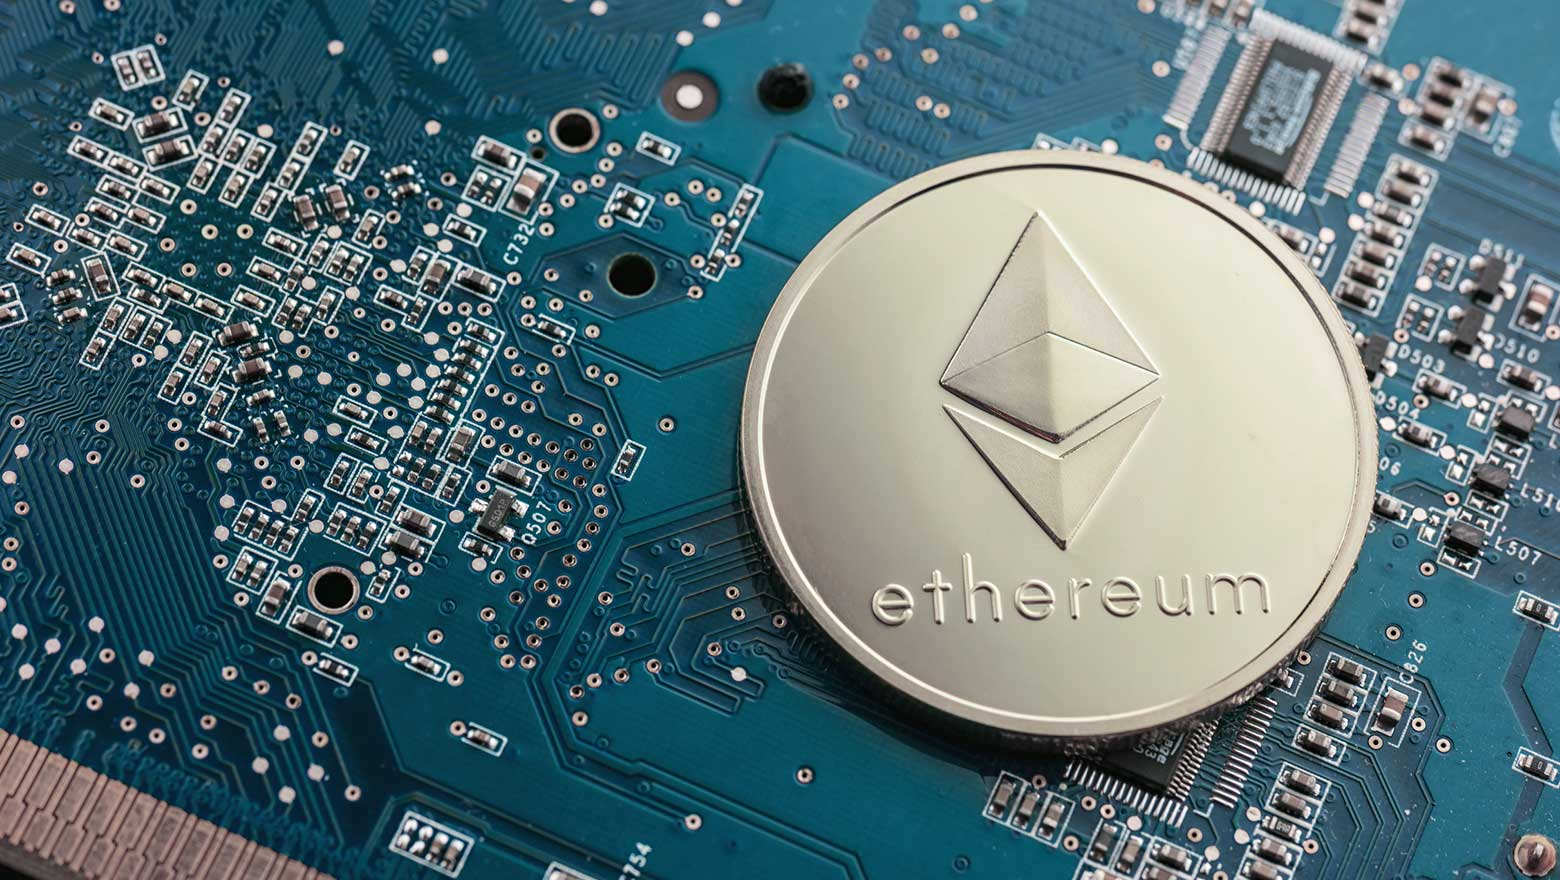
\includegraphics[width=0.55\textwidth]{resources/ethereum-crypto.jpg}
\end{figure}
Ethereum is the decentralized, open-source technology that powers much of the cryptocurrency world. Everything from decentralized finance applications and non-fungible tokens to enterprise blockchain solutions rely on Ethereum's technology. That has made Ethereum's native token, Ether, the second-largest cryptocurrency after Bitcoin.

The most direct option to have profit from the growing use of Ethereum is buying Ethereum cryptocurrency itself, but it can also be considered as store of value. Therefore there is a clear reason in desire to predict it's future prices.

For predictions we consider prices at the end of each week during last three years, in period from the January 1, 2019 till the beginning of 2022.

\section{Data exploration and transformation}%preparation, investigation
\subsection{The first look}
We start with plotting all the available data to have better understanding of time series we are working with (Fig.\ref{fig:raw_data}). We also split data, reserving last 10 weeks of observation for the test set.

\begin{figure}[h]
	\hspace{-1.5cm}
	\centering
	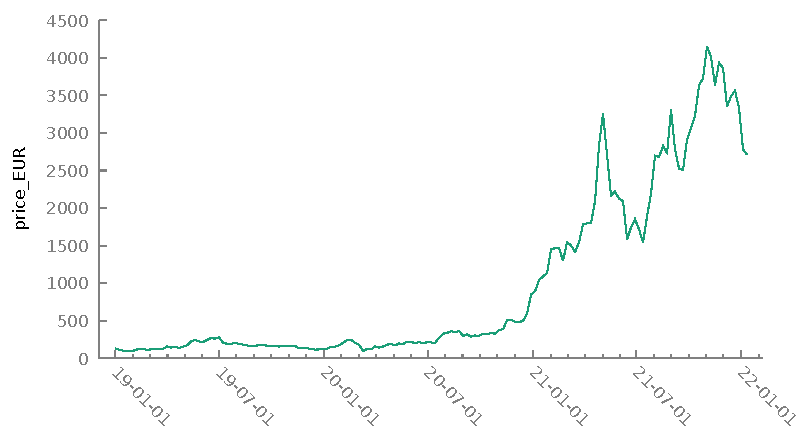
\includegraphics[width=0.55\textwidth]{resources/raw_data}
	\caption{History of the Ethereum prices.}
	\label{fig:raw_data}
\end{figure}
There is no obvious regularity in the data. Time series has no seasonal components, but we can easily notice a clear upgoing trend, with bigger jumps at the second half of the timeline. So we conclude process is not a stationary one. 

\subsection{Stationarity}
The assumption that our time series is a realization of a
stationary process is fundamental in time series
analysis. Thus, in order to construct an ARMA model, we must first
determine whether our time series can be considered a
realization of a stationary process.
%To be suitable for approximation with ARMA model, the time series should be stationary.
If initial data has no stationarity, we can achieve it throught specific transformations.

Mean of the process is not constant and getting bigger and bigger over time. Therefore, taking the first difference seems to be reasonable (Fig.\ref{fig:first_difference}).
\begin{figure}[h]
	\hspace{-1.5cm}
	\centering
	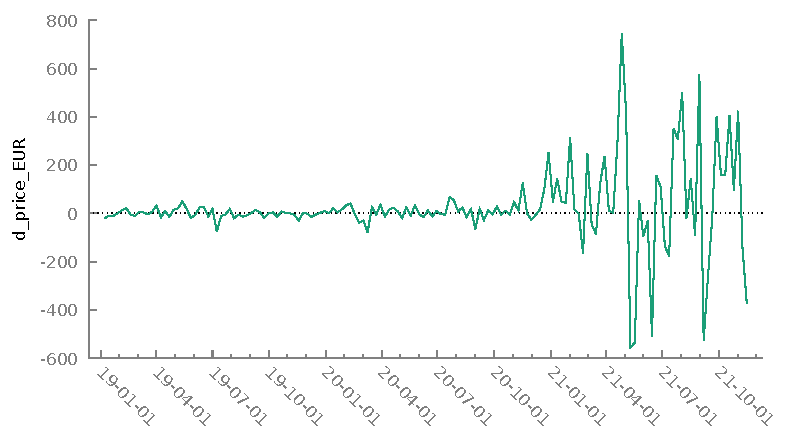
\includegraphics[width=0.7\textwidth]{resources/first_difference.pdf}
	\caption{The first difference.}
	\label{fig:first_difference}
\end{figure}

After the transformation we obtain the DGP with zero mean, as was expected, so we can proceed with the exploration.

Still, the process is not identically distributed because of high fluctuations in the second half of the timeline. To avoid this, we have to apply logarithmic function to the initial data. We will consider these data further in this work (Fig.\ref{fig:log}).

\begin{figure}[h]
    %\vspace{-1.5cm}
	\hspace{-1.5cm}
	\centering
	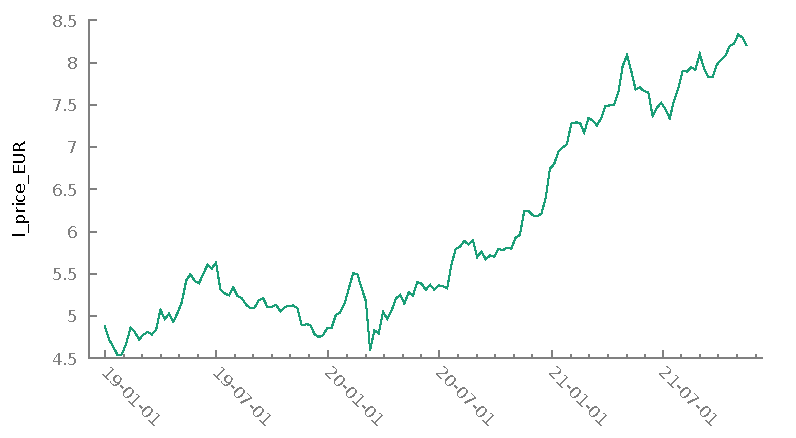
\includegraphics[width=0.7\textwidth]{resources/log.pdf}
	\caption{Logarithmized data.}
	\label{fig:log}
\end{figure}

%\newpage
What we observe is reduction of fluctuations in variance of the process, which allows us to take first difference again, but now based on logarithmic data (Fig.\ref{fig:log_difference}).

\begin{figure}[h]
	\hspace{-1.5cm}
	\centering
	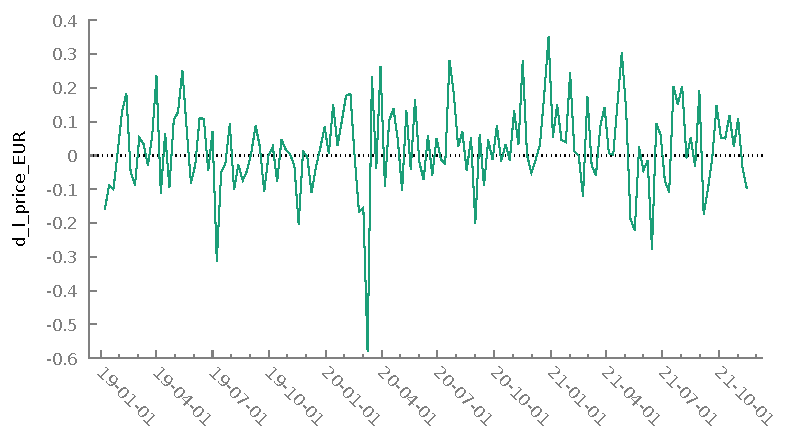
\includegraphics[width=0.7\textwidth]{resources/log_difference.pdf}
	\caption{First difference of the logs.}
	\label{fig:log_difference}
\end{figure}

\newpage
\subsection{Augmented Dickey-Fuller test}

Even thought the process might look like stationary, our conclusions may not be objective. As a last check of stationarity of the time series we consider the Augmented Dickey-Fuller test.
We assume that the time series has a unit root and then try to reject this hypothesis.
\begin{comment}
Augmented Dickey-Fuller test for d_l_price_EUR
testing down from 50 lags, criterion AIC
sample size 147
unit-root null hypothesis: a = 1

  test with constant 
  including 2 lags of (1-L)d_l_price_EUR
  model: (1-L)y = b0 + (a-1)*y(-1) + ... + e
  estimated value of (a - 1): -1.0459
  test statistic: tau_c(1) = -8.00371
  asymptotic p-value 4.875e-13
  1st-order autocorrelation coeff. for e: 0.019
  lagged differences: F(2, 143) = 3.714 [0.0268]

  with constant and trend 
  including 2 lags of (1-L)d_l_price_EUR
  model: (1-L)y = b0 + b1*t + (a-1)*y(-1) + ... + e
  estimated value of (a - 1): -1.0643
  test statistic: tau_ct(1) = -8.0339
  asymptotic p-value 1.504e-12
  1st-order autocorrelation coeff. for e: 0.019
  lagged differences: F(2, 142) = 3.843 [0.0237]
\end{comment}


After running the test, the unit root null-hypothesis was rejected.
As a result we got $p$-value near $1.5 \times 10^{-12} $ which is definitely less than $0.5$. So, indeed, the time series is stationary.

For the seek of comparison we also consider the Augmented Dickey-Fuller test for the time series on other steps of transformation (Table 1), which confirms our assumption about stationarity of other transformations, considered previously.

\begin{table}[h]
	\begin{center}
		\begin{tabular}{|c|c|c|c|c|}
			\hline
			
			\tabboxc{3cm}{}     
			& \tabboxc{3cm}{$p$-value}
			& \tabboxc{3cm}{is stationary?}
			\\ \hline
			
			raw data 
			& $1$
			& No
			\\ \hline
			
			logs              
			& $0.9834$
			& No
			\\ \hline
			
			first difference of logs
			& $1.5 \times 10^{-12} $
			& Yes
			\\ \hline
			
		\end{tabular}
		\caption{Results of Augmented Dickey-Fuller test.}
	\end{center}
\end{table}

\section{Model identification}
\subsection{Autocorrelation}
To identify a model, represented in the time series, we should first investigate, how values depend on each other. If we won't be able to spot any correlation, then there is no reason to proceed, because we won't be able to do any valuable prediction. 

Therefore it is useful to build correlogram (Fig. \ref{fig:correlogram}) with autocorrelation and partial autocorrelation functions. It also will help to identify the order of our ARMA model.

\begin{figure}[h!]
	\hspace{-1.5cm}
	\centering
	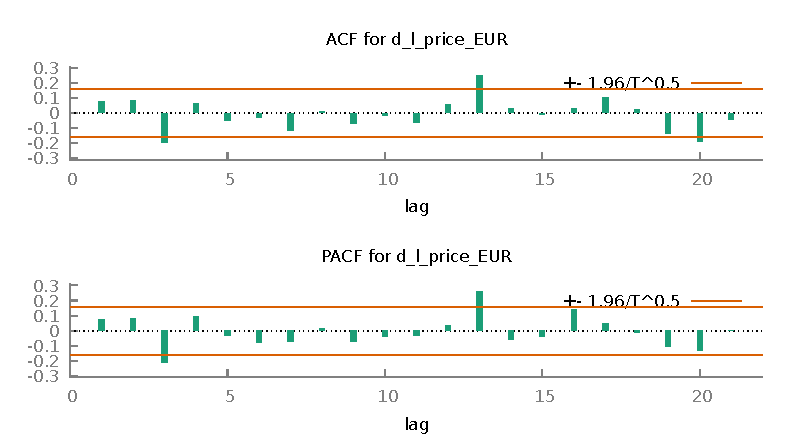
\includegraphics[width=0.7\textwidth]{resources/correlogram.pdf}
	\caption{The correlogram.}
	\label{fig:correlogram}
\end{figure}

Values at lags 3 and 13 are significantly different from zero. Luckily, we see the correlation, the process cannot be considered a realization of a white noise. The correlation is not significant, so it will be a bit tricky to predict values with high confidence, but we will try.

In advance we notice that MA model of order 3 might be a suitable realization of our process, but in general this case is difficult to interpret.

\subsection{Automatic criteria}

The mixed models can be particularly difficult to identify by
using the correlogram and the partial correlogram. For this reason, it is preferable to use information-based criteria such
as AIC, BIC or HQC. The AIC usually picks models which are over-parameterized.
The BIC is a criterion which attempts to correct the overfitting nature of the AIC.

Among a set of models, we select the values of p and q for our fitted model to be those which minimize these criteria. We analyze models from ARMA(0,0) to ARMA(13,13). The most valuable results are shown it the Table \ref{automatic-criteria}. 


\begin{comment}
? armax(10, 10, d_l_price_EUR, null, 1, 1, 0, 1, 0)
===============================================
 Information Criteria of ARMAX(p,q) for d_l_price_EUR
-----------------------------------------------
 p, q          AIC           BIC           HQC
-----------------------------------------------
 0, 0    -187.2606     -181.2662*    -184.8251 
 0, 1    -185.9914     -176.9997     -182.3381 
 0, 2    -186.0376     -174.0488     -181.1666 
 0, 3    -191.0878     -176.1017     -184.9990*
 0, 4    -189.5514     -171.5681     -182.2448 
 0, 5    -187.6091     -166.6286     -179.0847 
 0, 6    -186.2158     -162.2381     -176.4737 
 0, 7    -184.3880     -157.4131     -173.4282 
 0, 8    -182.3890     -152.4169     -170.2114 
 0, 9    -182.2047     -149.2354     -168.8093 
 0,10    -181.6595     -145.6929     -167.0463 
 1, 0    -186.1382     -177.1466     -182.4849 
 1, 1    -184.3182     -172.3294     -179.4472 
 1, 2    -189.6541     -174.6681     -183.5653 
 1, 3    -189.5617     -171.5784     -182.2551 
 1, 4    -187.5736     -166.5931     -179.0492 
 1, 5    -186.1668     -162.1891     -176.4247 
 1, 6    -184.4885     -157.5136     -173.5286 
 1, 7    -182.5101     -152.5380     -170.3325 
 1, 8    -180.5451     -147.5758     -167.1497 
 1, 9    -181.0283     -145.0617     -166.4151 
 1,10    -180.0689     -141.1051     -164.2380 
 2, 0    -185.1855     -173.1966     -180.3144 
 2, 1    -188.1568     -173.1708     -182.0680 
 2, 2    -190.0748     -172.0916     -182.7683 
 2, 3    -187.5407     -166.5602     -179.0164 
 2, 4    -185.8173     -161.8396     -176.0752 
 2, 5    -188.7767     -161.8018     -177.8168 
 2, 6    -190.8727     -160.9005     -178.6951 
 2, 7    -187.1585     -154.1892     -173.7631 
 2, 8    -187.1009     -151.1344     -172.4878 
 2, 9    -183.3930     -144.4293     -167.5621 
 2,10    -184.4309     -142.4699     -167.3822 
 3, 0    -189.7032     -174.7172     -183.6144 
 3, 1    -189.0582     -171.0750     -181.7517 
 3, 2    -188.0815     -167.1010     -179.5572 
 3, 3    -186.6223     -162.6446     -176.8802 
 3, 4    -184.7271     -157.7522     -173.7673 
 3, 5    -183.1045     -153.1324     -170.9269 
 3, 6    -182.1820     -149.2127     -168.7867 
 3, 7    -187.0054     -151.0388     -172.3923 
 3, 8    -184.3604     -145.3966     -168.5295 
 3, 9    -181.7513     -139.7903     -164.7027 
 3,10    -181.6220     -136.6639     -163.3556 
 4, 0    -189.1860     -171.2027     -181.8794 
 4, 1    -187.2401     -166.2596     -178.7158 
 4, 2    -185.6036     -161.6259     -175.8616 
 4, 3    -184.7756     -157.8007     -173.8158 
 4, 4    -183.1655     -153.1934     -170.9879 
 4, 5    -186.5614     -153.5921     -173.1661 
 4, 6    -185.8703     -149.9037     -171.2571 
 4, 7    -184.0264     -145.0626     -168.1955 
 4, 8    -182.4506     -140.4897     -165.4020 
 4, 9    -187.5902     -142.6320     -169.3238 
 4,10    -181.0087     -133.0533     -161.5245 
 5, 0    -187.3183     -166.3378     -178.7939 
 5, 1    -186.3959     -162.4182     -176.6538 
 5, 2    -191.4378*    -164.4629     -180.4779 
 5, 3    -187.3701     -157.3980     -175.1925 
 5, 4    -186.0427     -153.0734     -172.6473 
 5, 5    -184.0429     -148.0764     -169.4298 
 5, 6    -183.9223     -144.9585     -168.0914 
 5, 7    -184.5888     -142.6279     -167.5402 
 5, 8    -187.7132     -142.7550     -169.4468 
 5, 9    -185.9128     -137.9574     -166.4287 
 5,10    -185.8882     -134.9356     -165.1862 
 6, 0    -186.2697     -162.2920     -176.5276 
 6, 1    -184.9531     -157.9782     -173.9932 
 6, 2    -190.7491     -160.7770     -178.5715 
 6, 3    -188.7864     -155.8171     -175.3910 
 6, 4    -184.0428     -148.0762     -169.4297 
 6, 5    -185.4240     -146.4602     -169.5931 
 6, 6    -190.5337     -148.5727     -173.4850 
 6, 7    -187.4784     -142.5202     -169.2120 
 6, 8    -186.5133     -138.5579     -167.0292 
 6, 9    -185.9906     -135.0380     -165.2887 
 6,10    -185.5324     -131.5826     -163.6127 
 7, 0    -184.8301     -157.8552     -173.8702 
 7, 1    -182.9824     -153.0103     -170.8048 
 7, 2    -181.1084     -148.1391     -167.7131 
 7, 3    -184.0420     -148.0754     -169.4288 
 7, 4    -189.0080     -150.0442     -173.1771 
 7, 5    -182.4146     -140.4536     -165.3660 
 7, 6    -187.3520     -142.3938     -169.0856 
 7, 7    -186.5788     -138.6234     -167.0946 
 7, 8    -184.8722     -133.9196     -164.1703 
 7, 9    -186.9274     -132.9776     -165.0077 
 7,10    -184.9999     -128.0528     -161.8624 
 8, 0    -182.8428     -152.8707     -170.6652 
 8, 1    -180.9831     -148.0138     -167.5878 
 8, 2    -179.1726     -143.2061     -164.5595 
 8, 3    -182.0491     -143.0854     -166.2182 
 8, 4    -187.5642     -145.6032     -170.5155 
 8, 5    -184.2048     -139.2466     -165.9384 
 8, 6    -188.8413     -140.8859     -169.3572 
 8, 7    -184.6055     -133.6529     -163.9035 
 8, 8    -182.5419     -128.5921     -160.6222 
 8, 9    -185.7129     -128.7658     -162.5754 
 8,10    -183.8308     -123.8865     -159.4756 
 9, 0    -181.9105     -148.9412     -168.5152 
 9, 1    -180.1145     -144.1480     -165.5014 
 9, 2    -187.1175     -148.1537     -171.2866 
 9, 3    -183.4706     -141.5096     -166.4219 
 9, 4    -186.2510     -141.2928     -167.9846 
 9, 5    -183.6401     -135.6847     -164.1559 
 9, 6    -187.0145     -136.0619     -166.3126 
 9, 7    -185.2087     -131.2589     -163.2890 
 9, 8    -183.1696     -126.2226     -160.0322 
 9, 9    -183.9334     -123.9892     -159.5782 
 9,10    -181.9640     -119.0225     -156.3910 
10, 0    -180.2033     -144.2368     -165.5902 
10, 1    -178.2152     -139.2514     -162.3843 
10, 2    -185.1183     -143.1573     -168.0697 
10, 3    -185.6652     -140.7070     -167.3988 
10, 4    -184.9708     -137.0154     -165.4867 
10, 5    -184.1100     -133.1574     -163.4081 
10, 6    -185.0896     -131.1398     -163.1699 
10, 7    -183.2639     -126.3168     -160.1264 
10, 8    -181.6513     -121.7071     -157.2961 
10, 9    -181.9892     -119.0477     -156.4162 
10,10    -182.0011     -116.0624     -155.2104 
===============================================
* indicates best models.
'9999.9999' suggests failures to estimate the models.
\end{comment}

\begin{table}[h]
	\begin{center}
		\begin{tabular}{|c|c|c|c|c|}
			\hline
			
			\tabboxc{1cm}{AR}     
			& \tabboxc{1cm}{MA}
			& \tabboxc{3cm}{AIC}
			& \tabboxc{3cm}{BIC}
			& \tabboxc{3cm}{HQC}
			\\ \hline
			
			0 
			& 0
			& -187.2606
			& \textbf{-181.2662}
			& -184.8251
			\\ \hline
			
			0          
			& 1
			& -185.9914
			& -176.9997
			& -182.3381
			\\ \hline
			
			1               
			& 0
			& -186.1382
			& -177.1466
			& -182.4849
			\\ \hline
			
			0
			& 3
			& -191.0878
			& -176.1017
			& \textbf{-184.9990}
			\\ \hline
			
			3
			& 0
			& -189.7032
			& -174.7172
			& -183.6144
			\\ \hline
			
			5             
			& 2
			& \textbf{-191.4378}
			& -164.4629
			& -180.4779
			\\ \hline
		\end{tabular}
		\caption{The automatic criteria test}
		\label{automatic-criteria}
	\end{center}
\end{table}

The BIC criterion warns us that our process might be a realization of white noise. However, other criteria, AIC and HQC, propose different, MA(3) and ARMA(5, 2) models respectively, which we are going to estimate. After estimation of all the parameters, we should verify if the model is a good representation of our data. 


\section{Models evaluation}
To check if the model fits data well, we have to calculate the residuals and then consider their properties.
From theory we know that if the model chosen is
correct and if the estimated parameters are close to the
actual values, then the residuals should be a realization of a
white noise.

\subsection{ARIMA(0,1,3)}
Firstly, let's evaluate ARIMA(0,1,3) model, which is MA(3) on first difference. We build the residual correlogram to identify, if there is any correlation between residuals (Fig. \ref{fig:ma_3_residual_corr}).

\begin{figure}[h!]
%\vspace{-1cm}
	\centering
	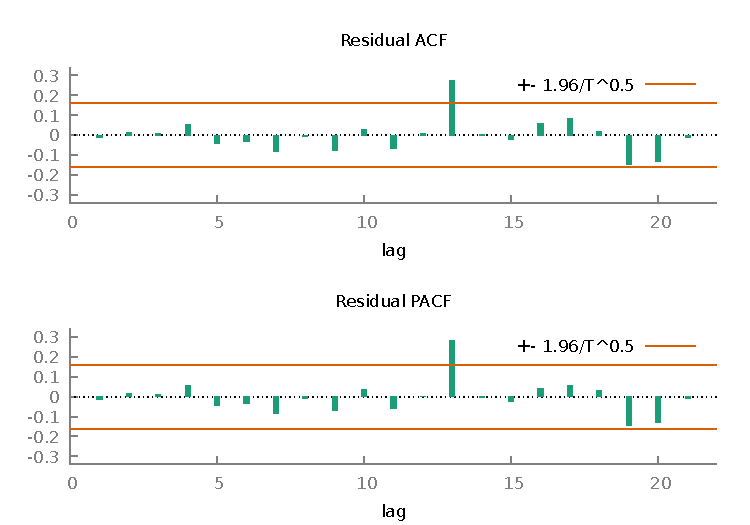
\includegraphics[height=0.3\textheight, width=0.7\textwidth]{resources/ma_3_residual_corr.pdf}
    \caption{The residual correlogram for the ARIMA(0,1,3) model.}
	\label{fig:ma_3_residual_corr}
\end{figure}

At first lags we see absolutely no correlation between residuals and only one value at lag 13 is significantly different from zero. So, at some point, it can be considered a realization of a white noise.
The same conclusion may be done from Q-statistics plot (Fig. \ref{fig:qq_residual}): %(Fig.\ref{fig:qq_residual}).

\begin{figure}[h!]
%\vspace{-2cm}
	\centering
	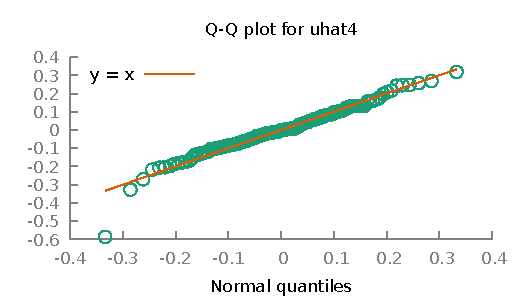
\includegraphics[width=0.7\textwidth]{resources/qq_residual.pdf}
	\caption{The residual Q-Q plot for the ARIMA(0,1,3) model.}
	\label{fig:qq_residual}
\end{figure}

It is not clear, what to do with that one anomaly at lag 13. Therefore we should check if residuals' distribution is a realization of Gaussian white noise. After testing it for normality we get results, shown on Fig. \ref{fig:residuals_normality}.

\begin{figure}[h!]
	\centering
	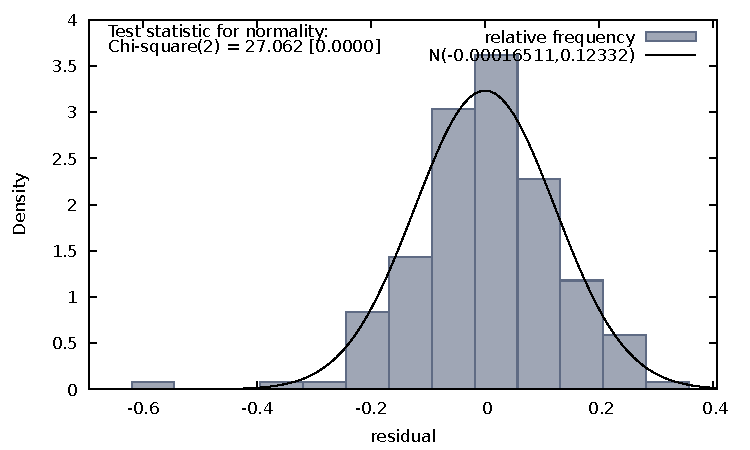
\includegraphics[width=0.7\textwidth]{resources/residuals_normality.pdf}
	\caption{The residuals' normality test for the ARIMA(0,1,3) model.}
	\label{fig:residuals_normality}
\end{figure}

It is clear that the distribution is not a Gaussian one, so, theoretically, the ARIMA(0,1,3) model is not a good choice for our time series. We can also see this from the model forecast on Fig. \ref{fig:ma3forecast}. 

\begin{figure}[h!]
	\centering
	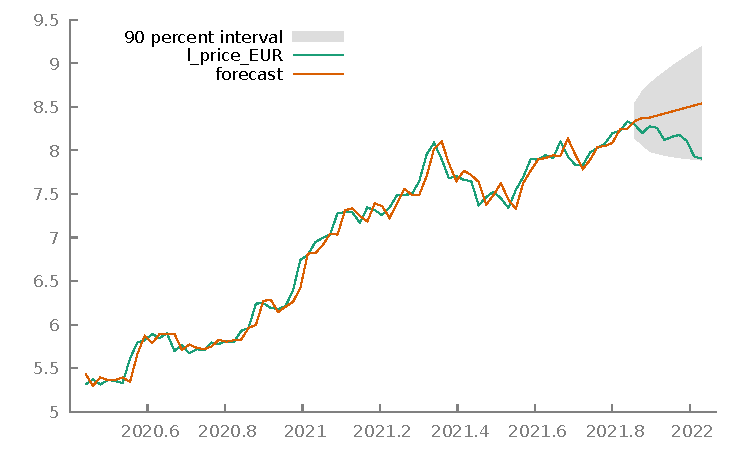
\includegraphics[width=0.7\textwidth]{resources/ma3forecast.pdf}
	\caption{The forecast based on ARIMA(0,1,3) model.}
	\label{fig:ma3forecast}
\end{figure}

\subsection{ARIMA(5,1,2)}
Secondly, let's evaluate ARIMA(5,1,2) model, which is ARMA(5,2) on first difference. As usual, we consider the residuals' correlogram on Fig. \ref{fig:arma_5_2_residual_corr}.

\begin{figure}[h!]
	\centering
	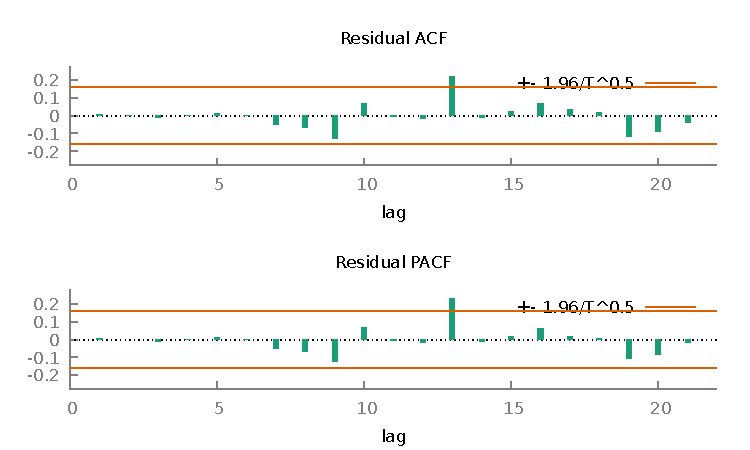
\includegraphics[width=0.7\textwidth]{resources/arma_5_2_residual_corr.pdf}
	\caption{The residual correlogram for the ARIMA(5,1,2) model.}
	\label{fig:arma_5_2_residual_corr}
\end{figure}

It has the same issue at lag 13, as the previous model, but with much smaller value. After testing it for normality we get analogical results (Fig. \ref{fig:residual_normality2}).

\begin{figure}[h!]
	\centering
	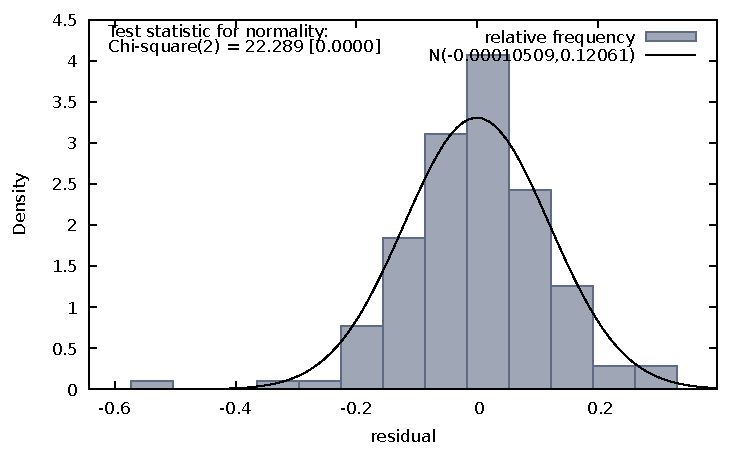
\includegraphics[width=0.7\textwidth]{resources/residual_normality2.pdf}
	\caption{The residuals' normality test for the ARIMA(5,1,2) model.}
	\label{fig:residual_normality2}
\end{figure}

Unfortunately, it is also not a Gaussian distribution and model is not a good approximation of our data. Predictions of this model looks like on Fig. \ref{fig:arma52forecast}.

\begin{figure}[H]
	\centering
	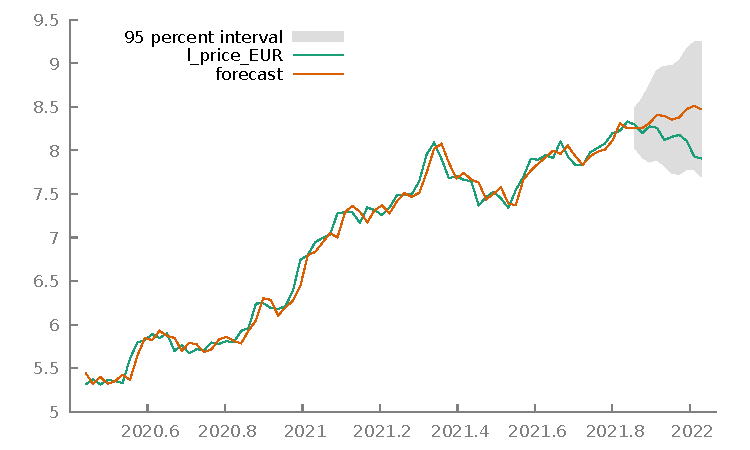
\includegraphics[width=0.7\textwidth]{resources/arma52forecast.pdf}
	\caption{The forecast based on ARIMA(5,1,2) model.}
	\label{fig:arma52forecast}
\end{figure}

Generally speaking, we obtain similar results from few other ARIMA models. This is a reason to draw a conclusion that it is hard to obtain good approximation for the chosen time series.




\subsection{Comparison}


To compare performance of these two models, we should consider root mean squared error. It also makes sense to compare predictions with white noise based one, to see if any of the models is efficient at all.

\begin{table}[h]
	\begin{center}
		\begin{tabular}{|c|c|c|}
			\hline
			
			\tabboxc{4cm}{Model}     
			& \tabboxc{6cm}{Root Mean Squared Error}
			\\ \hline
			
			white noise
			& 0.36843 
			\\ \hline
			
			ARIMA(0,1,3)         
			& 0.34833 
			\\ \hline
			
			ARIMA(5,1,2)              
			& \textbf{0.3117}
			\\ \hline
			
		\end{tabular}
		\caption{Models' error comparison.}
		\label{rmse}
	\end{center}
\end{table}


We see that both models performs better than "random" predictions.
The ARIMA(5,1,2) has lower RMSE than ARIMA(0,1,3), but it is also more complex, with bigger number of parameters, which means that there is a risk of overfitting.

Both models predict future not very well and this is most likely related to the almost random nature of the time series. But if we have to choose, than it is suitable to say that ARIMA(5,1,2) model represents the data distribution better.

\section{Conclusion}
As we can see, predicting future is definitely not an easy task.
A reliable ARMA time series forecast requires that the future is not
too different from the past. Therefore, poor performance might be related to the nature of the time series, which in our case was very similar to the stock data.

Even if we are able to build the appropriate model, usually there is no sense to consider predictions for long time periods as valuable. If one have to use such models in a real world, a good strategy is to retrain the model at the end of time interval, when new data is available, to maintain maximum possible accuracy.

The flexibility of ARMA models can be distinguished as one of the advantages, in a row with ability to forecast data without impact of side conditions. On other hand, it requires large number of observations for model identification, estimation and training. Also it cannot stand against structural changes of the data.

As a result we may sum up that ARMA model predictions not always may be considered as reliable, but they play important role for us to understand the data and the environment better.


\end{document}
